\subsubsection{NASA-TLX}
\label{subsubsec:results_nasa_tlx_2}

\paragraph{Analysis of the mental demand scale}\mbox{}\\

The Table \ref{tab:md_table_noBase} presents the ‘mental demand’ score of all participants, while the corresponding barplot is presented in Figure \ref{fig:barplot_md_avg_4_scene_blind_sight}. It is interesting to observe that sighted people gave a higher score to audio, as they are not so familiar to use sounds as source of guidance.


\begin{table}[!htb]
\centering
\caption{Mental demand felled by the participants.}
\label{tab:md_table_noBase}
\begin{tabular}{lllrrrrr}
\toprule
    &       &        & Audio & \begin{tabular}[c]{@{}l@{}}Haptic\\ Belt\end{tabular} & \begin{tabular}[c]{@{}l@{}}Virtual\\ Cane\end{tabular} & Mixture \\
Participant & \begin{tabular}[c]{@{}l@{}}Visual\\ Condition\end{tabular} & Round &       &                                                       &                                                        &         \\
\midrule
001 & Sight & First &    12 &                                                    11 &                                                      5 &       9 \\
    &       & Return &    13 &                                                    13 &                                                      5 &      10 \\
001C & Blind & First &     1 &                                                    14 &                                                      3 &       6 \\
    &       & Return &     1 &                                                    10 &                                                      2 &       6 \\
002C & Blind & First &     1 &                                                     1 &                                                     10 &      12 \\
    &       & Return &     1 &                                                     1 &                                                     10 &       3 \\
003 & Sight & First &    18 &                                                    18 &                                                     16 &      10 \\
    &       & Return &    12 &                                                    15 &                                                     11 &       8 \\
003C & Blind & First &     5 &                                                     5 &                                                      8 &       1 \\
    &       & Return &     1 &                                                     1 &                                                      2 &       1 \\
004 & Sight & First &    17 &                                                    20 &                                                     12 &      20 \\
    &       & Return &    12 &                                                    15 &                                                     10 &      15 \\
004C & Blind & First &    10 &                                                    15 &                                                     10 &      10 \\
    &       & Return &    10 &                                                    14 &                                                      8 &      10 \\
005 & Sight & First &     4 &                                                    12 &                                                     10 &      13 \\
    &       & Return &     6 &                                                    10 &                                                      6 &      12 \\
\bottomrule
\end{tabular}
\end{table}



 %The Figures \ref{fig:barplot_md_avg_4_scene_blind} and \ref{fig:barplot_md_avg_4_scene_sight} show a systematic reduction on the perceived mental demand in all methods between the rounds for both groups. But the Figure \ref{fig:barplot_md_avg_4_scene} shows that the average of each method was very different between the two groups.

\begin{figure}[!htb]
    \centering
    \begin{minipage}{\textwidth}
        \centering
        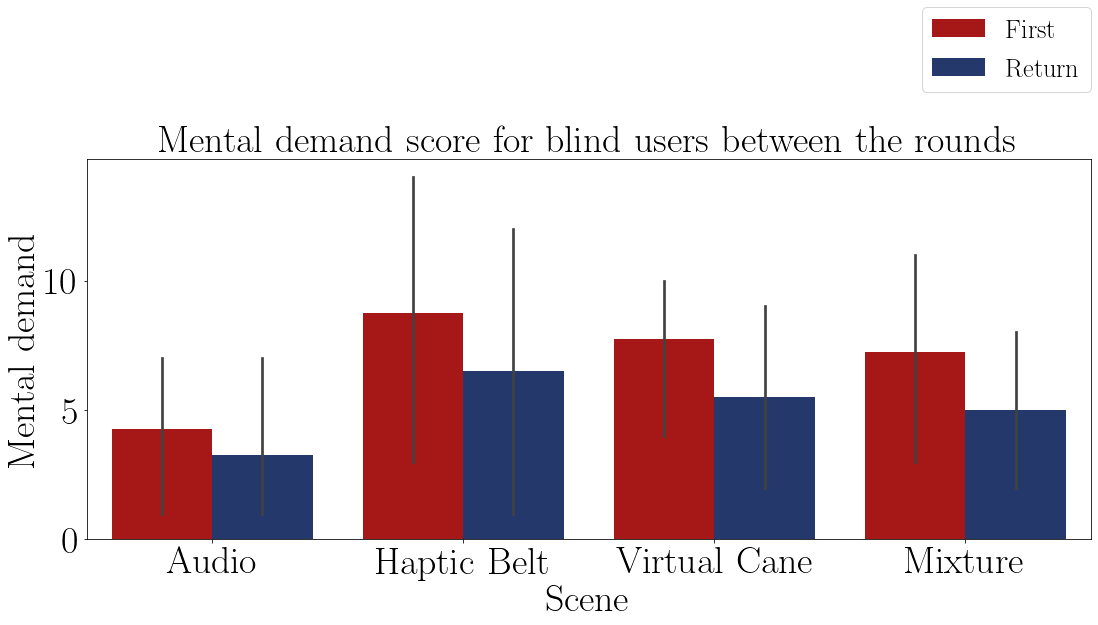
\includegraphics[width = 0.8\linewidth]{Resultados/Nasa/Figuras/png/barplot_md_avg_4_scene_blind.png}
        \subcaption{Blind participants}
        \label{fig:barplot_md_avg_4_scene_blind}
    \end{minipage}
    \begin{minipage}{\textwidth}
        \centering
        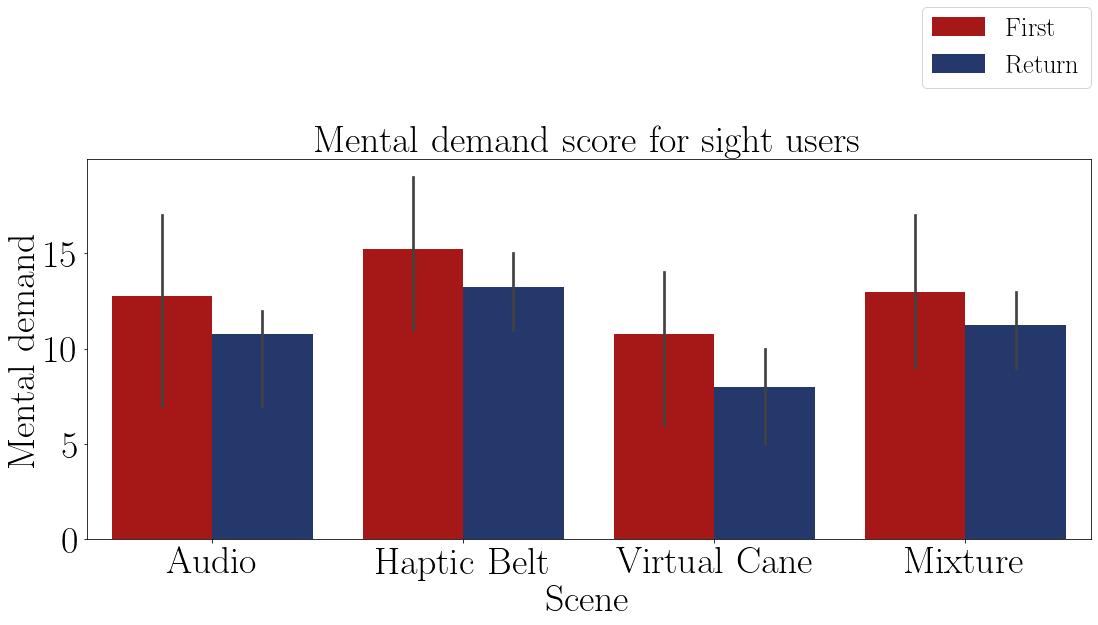
\includegraphics[width = 0.8\linewidth]{Resultados/Nasa/Figuras/png/barplot_md_avg_4_scene_sight.png}
        \subcaption{Sight participants}
        \label{fig:barplot_md_avg_4_scene_sight}
    \end{minipage}
    \caption{Barplot of the average mental demand on each method and round.}
    \label{fig:barplot_md_avg_4_scene_blind_sight}
\end{figure}
%\begin{figure}[!htb]
%    \centering
%    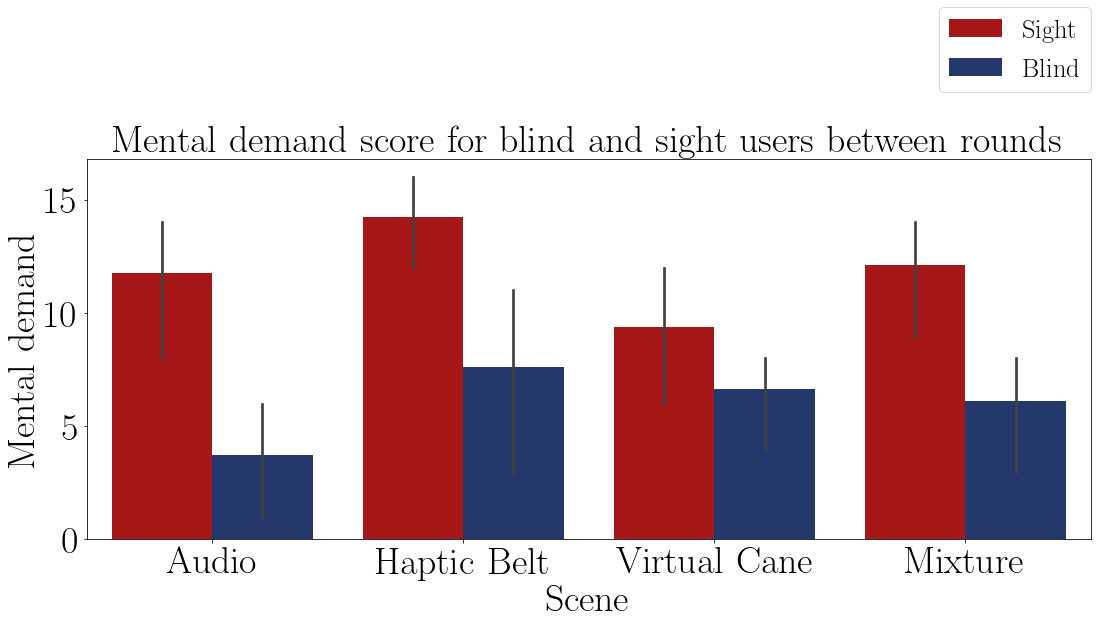
\includegraphics[width = 0.8\linewidth]{Resultados/Nasa/Figuras/png/barplot_md_avg_4_scene.png}
%    \caption{Barplot of the average mental demand of both participants on each method.}
%    \label{fig:barplot_md_avg_4_scene}
%\end{figure}

Figures \ref{fig:boxplot_noBase_md_4_scene} and \ref{fig:boxplot_noBase_md_4_rounds} presents the box plot for both groups, organized by method and round. It is clear that the mental demand is systematically higher for sighted people, which is something expected. But while blind participants considered the ‘audio’ method less demanding, sighted participants gave preference to the virtual cane. For both groups, we observe a decrease in the mental demand.

\begin{figure}[!htb]
    \centering
    \begin{minipage}{0.45\textwidth}
        \centering
        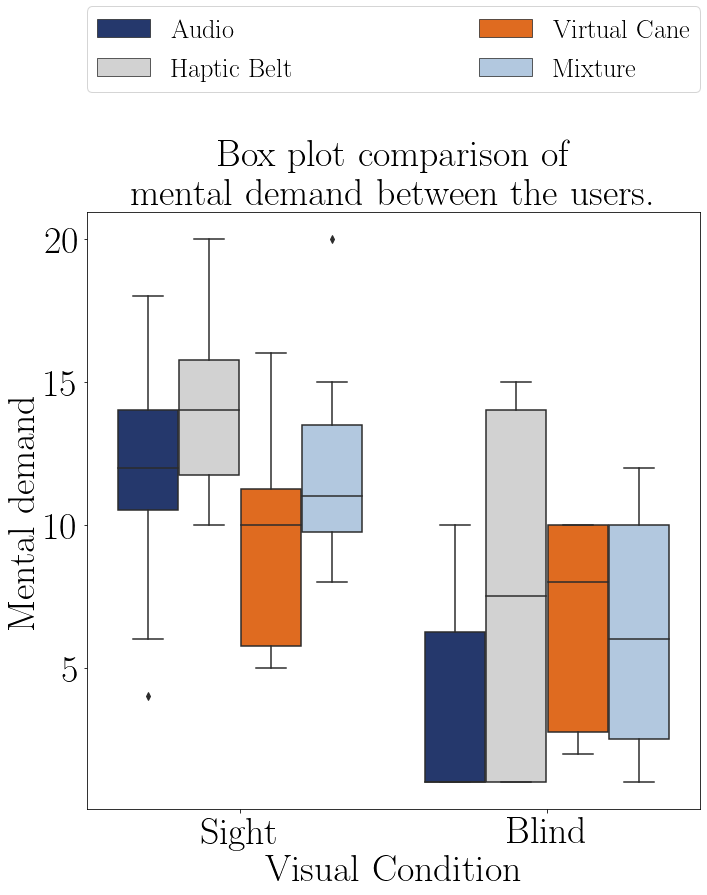
\includegraphics[width = 0.8\linewidth]{Resultados/Nasa/Figuras/png/boxplot_noBase_md_4_scene.png}
        \caption{Boxplot of the mental demand of the participants grouped by method.}
        \label{fig:boxplot_noBase_md_4_scene}
    \end{minipage}
    \begin{minipage}{0.45\textwidth}
        \centering
        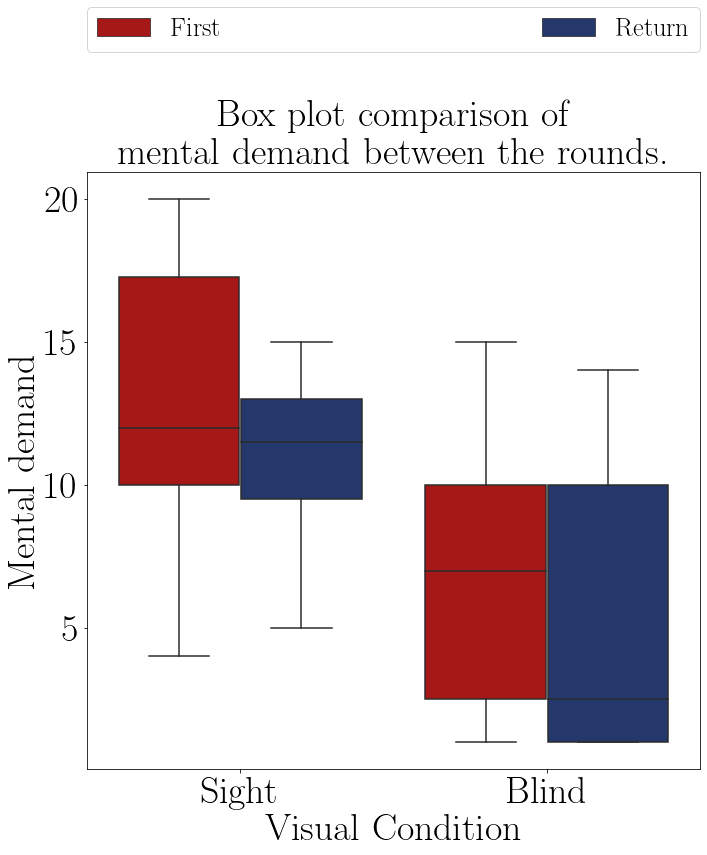
\includegraphics[width = 0.8\linewidth]{Resultados/Nasa/Figuras/png/boxplot_noBase_md_4_rounds.png}
        \caption{Boxplot of the mental demand of the participants grouped by round.}
        \label{fig:boxplot_noBase_md_4_rounds}
    \end{minipage}
\end{figure}

%The Table \ref{tab:md_average_group_noBase} shows the average mental demand of both samples and is possible to notice how the average perceived mental demand by the sight sample was higher in every method.
%
%
\begin{table}[!htb]
\centering
\caption{Mental demand average grouped by participant and visual condition}
\label{tab:md_average_group_noBase}
\begin{tabular}{lrrrrrr}
\toprule
{} &  Audio & \begin{tabular}[c]{@{}l@{}}Haptic\\ Belt\end{tabular} & \begin{tabular}[c]{@{}l@{}}Virtual\\ Cane\end{tabular} &  Mixture \\
Visual Condition &        &                                                       &                                                        &          \\
\midrule
Blind            &   3.75 &                                                  7.62 &                                                   6.62 &    6.125 \\
Sight            &  11.75 &                                                 14.25 &                                                   9.38 &   12.125 \\
\bottomrule
\end{tabular}
\end{table}



Figures \ref{fig:qqplot_md_avg_two_way_sight} and \ref{fig:residplot_md_avg_two_way_sight} show the QQ plot and residual distribution for the sighted data, confirming that the data is normally distributed and participants have similar variance. Table \ref{tab:blocanova_md_avg_two_way_blind_sight} brings the results of ANOVA. Different from the blind participants, in the case of sighted ones, the p-value for ‘method’ is below the threshold of 0.05, confirming it as a significant variable for the mental demand. In the case of ‘round’, data from both sighted and blind participants resulted in the same p-value of 0.075, which is close to the traditional threshold of 0.05, but slightly higher. 

\begin{table}
    \caption{Anova p-value for the mental demand average on each method'}
    \label{tab:blocanova_md_avg_two_way_blind_sight}
\begin{minipage}{0.45\textwidth}
    \subcaption{Blind participants}
    
\centering
\begin{tabular}{ll}
\toprule
          Source & P-Value \\
\midrule
    \    Methods &   0.170 \\
     \    Rounds &   0.075 \\
\    Interaction &   0.993 \\
\bottomrule
\end{tabular}

\end{minipage}
\begin{minipage}{0.45\textwidth}
    \subcaption{Sight participants}
    
\centering
\begin{tabular}{ll}
\toprule
          Source & P-Value \\
\midrule
    \    Methods & 0.049** \\
     \    Rounds &   0.075 \\
\    Interaction &   0.990 \\
\bottomrule
\end{tabular}
    
\end{minipage}
\end{table}

\begin{figure}[!htb]
    \centering
    \begin{minipage}{0.45\textwidth}
        \centering
        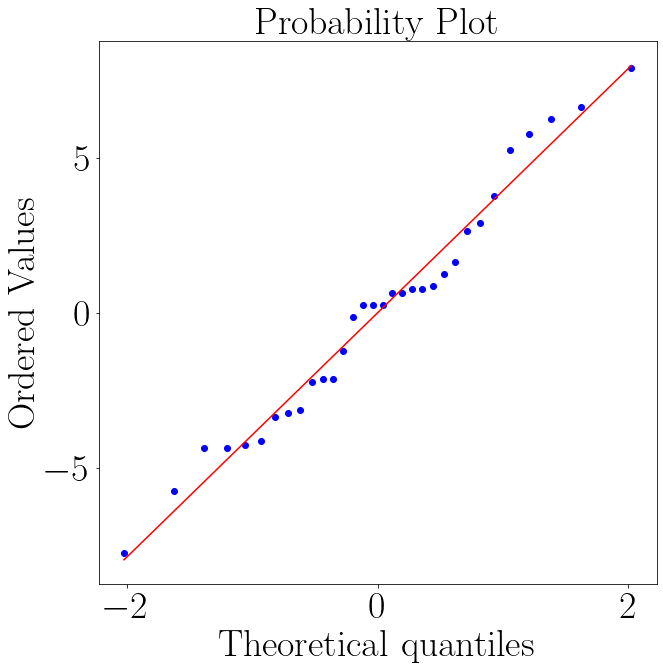
\includegraphics[width = 0.8\linewidth]{Resultados/Nasa/Figuras/png/qqplot_md_avg_two_way_sight.png}
        \caption{QQ plot of the mental demand of the sight participants on each method.}
        \label{fig:qqplot_md_avg_two_way_sight}
    \end{minipage}
    \begin{minipage}{0.45\textwidth}
        \centering
        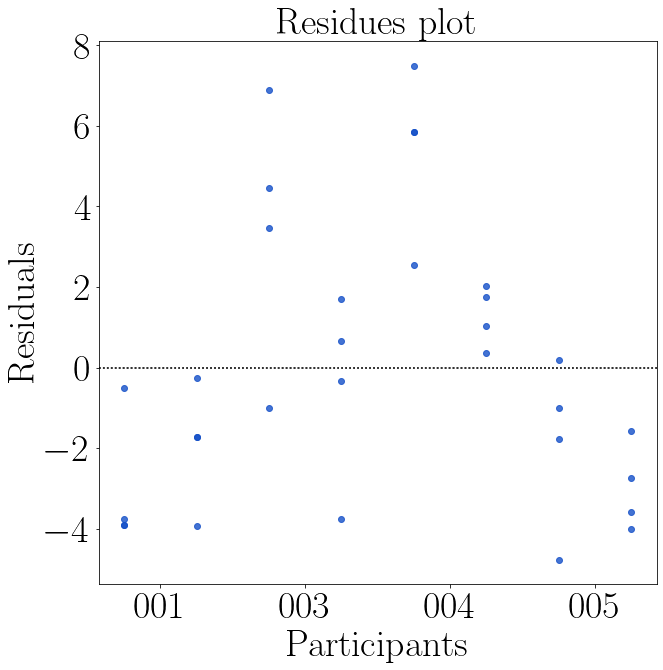
\includegraphics[width = 0.8\linewidth]{Resultados/Nasa/Figuras/png/residplot_md_avg_two_way_sight.png}
        \caption{Residual plot of the mental demand score the sighted participants on each method.}
        \label{fig:residplot_md_avg_two_way_sight}
    \end{minipage}
\end{figure}

%The Table \ref{tab:lsd_md_avg_two_way_sight} presents the conclusion of a pairwise Fisher LSD test of the previous ANOVA test. The results show that only the "Audio" has a similar mental demand as the "Mixture" method.
%
%
\begin{table}[!htb]
\centering
\caption{Cross validation p-value for the mental demand average on each method for sighted users.}
\label{tab:lsd_md_avg_two_way_sight}
\begin{tabular}{rcllr}
\toprule
      \multicolumn{3}{c}{Method} &                          \multicolumn{2}{c}{Analysis} \\
\midrule
       Audio & $X$ & Haptic Belt &        $H_1 : \mu_{Audio} \ne \mu_{Haptic Belt}$ & ** \\
      Audio & $X$ & Virtual Cane &       $H_1 : \mu_{Audio} \ne \mu_{Virtual Cane}$ & ** \\
           Audio & $X$ & Mixture &                $H_0 : \mu_{Audio} = \mu_{Mixture}$ &  \\
Haptic Belt & $X$ & Virtual Cane & $H_1 : \mu_{Haptic Belt} \ne \mu_{Virtual Cane}$ & ** \\
     Haptic Belt & $X$ & Mixture &      $H_1 : \mu_{Haptic Belt} \ne \mu_{Mixture}$ & ** \\
    Virtual Cane & $X$ & Mixture &     $H_1 : \mu_{Virtual Cane} \ne \mu_{Mixture}$ & ** \\
\bottomrule
\end{tabular}
\end{table}


%
%The Table \ref{tab:md_var_average_group} shows the average of the mental demand variation between the rounds. This table shows that the mental demand variation from the “Audio” has the lower variation, and the rest are similar variations.
%
%
\begin{table}[!htb]
\centering
\caption{Mental demand variation grouped by participant and visual Condition}
\label{tab:md_var_average_group}
\begin{tabular}{lrrrrrr}
\toprule
{} &     Base &    Audio & \begin{tabular}[c]{@{}l@{}}Haptic\\ Belt\end{tabular} & \begin{tabular}[c]{@{}l@{}}Virtual\\ Cane\end{tabular} &  Mixture \\
Visual Condition &          &          &                                                       &                                                        &          \\
\midrule
Blind            &  -52.2\% &  -20.0\% &                                               -28.8\% &                                                -32.1\% &  -18.750 \\
Sight            &  -21.9\% &   -1.1\% &                                               -10.0\% &                                                -22.0\% &  -10.395 \\
\bottomrule
\end{tabular}
\end{table}


%
%The Figures \ref{fig:qqplot_md_var_sight} and \ref{fig:residplot_md_var_sight} shows the distribution and variance of the mental demand variation of the Table \ref{tab:md_table_blind}. These Figures shows that the data are normally distributed and that the methods have a similar variance.
%The Table \ref{tab:blocanova_md_var_sight} shows the Anova test p-value of the mental demand of the "sight" sample between the guidance methods. The p-value indicates that there is no influence of the methods in the variation of mental demand between the rounds. 
%
%
\begin{table}[!htb]
\centering
\caption{Anova p-value for the mental demand variation on each method for sighted users.}
\label{tab:blocanova_md_var_sight}
\begin{tabular}{lrrrrr}
\toprule
               Source &  Squared sum &  DOF & Squared average &     F & \begin{tabular}[c]{@{}l@{}}P-Value \\ $(F_{0} > F)$\end{tabular} \\
\midrule
Participants (blocks) &       74.250 &    3 &           0.750 & 6.319 &                                                                  \\
               Method &        2.250 &    3 &          24.750 & 0.191 &                                                            0.900 \\
   Experimental error &       35.250 &    9 &           3.917 &       &                                                                  \\
                Total &      111.750 &   15 &                 &       &                                                                  \\
\bottomrule
\end{tabular}
\end{table}


%
%\begin{figure}[!htb]
%    \centering
%    \begin{minipage}{0.45\textwidth}
%        \centering
%        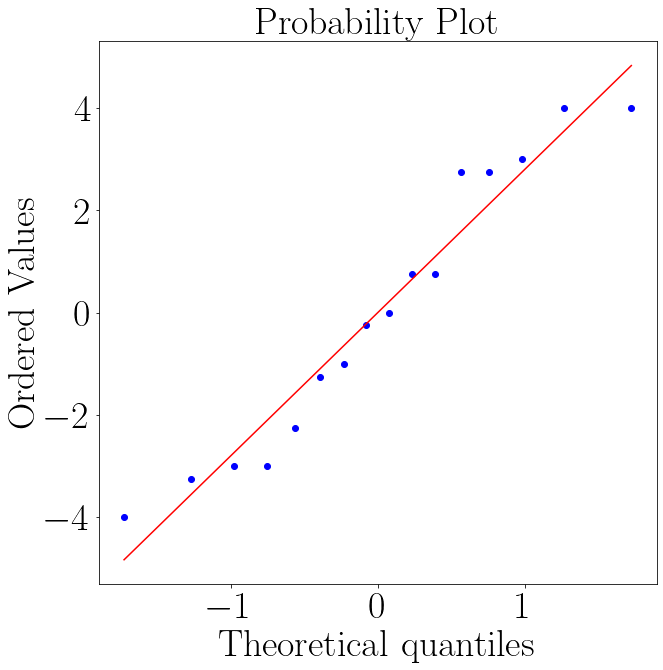
\includegraphics[width = 0.8\linewidth]{Resultados/Nasa/Figuras/png/qqplot_md_var_sight.png}
%        \caption{Residual plot of the mental demand variation of the blind participants on each method.}
%        \label{fig:qqplot_md_var_sight}
%    \end{minipage}
%    \begin{minipage}{0.45\textwidth}
%        \centering
%        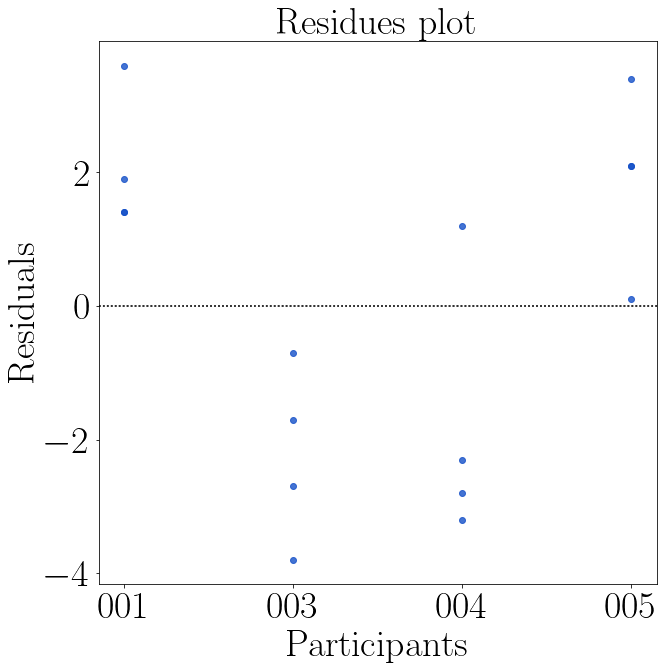
\includegraphics[width = 0.8\linewidth]{Resultados/Nasa/Figuras/png/residplot_md_var_sight.png}
%        \caption{Residual plot of the mental demand variation of the sighted participants on each method.}
%        \label{fig:residplot_md_var_sight}
%    \end{minipage}
%\end{figure}
%
%%The Table \ref{tab:lsdbloc_mental_demand_var} presents the conclusion of a pairwise Fisher LSD test of the blind mental demand between all the guidance methods. The results show that all methods have similar variations.
%
%%
\begin{table}[!htb]
\centering
\caption{Cross validation p-value for the mental demand variation on each method for blinded users.}
\label{tab:lsdbloc_mental_demand_var}
\begin{tabular}{rclr}
\toprule
      \multicolumn{3}{c}{Method} &                                       Analysis \\
\midrule
              Base & $X$ & Audio &           $H_1 : \mu_{Base} \ne \mu_{Audio}**$ \\
        Base & $X$ & Haptic Belt &         $H_0 : \mu_{Base} = \mu_{Haptic Belt}$ \\
       Base & $X$ & Virtual Cane &    $H_1 : \mu_{Base} \ne \mu_{Virtual Cane}**$ \\
            Base & $X$ & Mixture &         $H_1 : \mu_{Base} \ne \mu_{Mixture}**$ \\
       Audio & $X$ & Haptic Belt &    $H_1 : \mu_{Audio} \ne \mu_{Haptic Belt}**$ \\
      Audio & $X$ & Virtual Cane &       $H_0 : \mu_{Audio} = \mu_{Virtual Cane}$ \\
           Audio & $X$ & Mixture &            $H_0 : \mu_{Audio} = \mu_{Mixture}$ \\
Haptic Belt & $X$ & Virtual Cane & $H_0 : \mu_{Haptic Belt} = \mu_{Virtual Cane}$ \\
     Haptic Belt & $X$ & Mixture &  $H_1 : \mu_{Haptic Belt} \ne \mu_{Mixture}**$ \\
    Virtual Cane & $X$ & Mixture &     $H_0 : \mu_{Virtual Cane} = \mu_{Mixture}$ \\
\bottomrule
\end{tabular}
\end{table}


%
%To close up, according to the ANOVA test at Table \ref{tab:lsd_md_avg_two_way_sight} the method do have influence on the mental demand of the sighted participant and that the "Audio" and the "Mixture" method have the same mental demand for them. This differs from the result of the previous section that was the ANOVA did not prove any effect and that the "Audio" and "Mixture" methods could not be said to be similar. Although for the "blind" users, they were also the methods that caused the lowest mental demand.
%
%There is no influence in the tested methods in the participants mental demand variation, as shown in the Table \ref{tab:blocanova_md_var_sight}.

\FloatBarrier

%%%%%%%%%%%%%%%%%%%%%%%%%%%%%%%%%%%%%%%%%%%%%%%%%%%%%%%%%%%%%%%%%%%%%%%%%%%%
%%%%%%%%%%%%%%%%%%%%%%%%%%%%%%%%%%%%%%%%%%%%%%%%%%%%%%%%%%%%%%%%%%%%%%%%%%%%
%%%%%%%%%%%%%%%%%%%%%%%%%%%%%%%%%%%%%%%%%%%%%%%%%%%%%%%%%%%%%%%%%%%%%%%%%%%%
%%%%%%%%%%%%%%%%%%%%%%%%%%%%%%%%%%%%%%%%%%%%%%%%%%%%%%%%%%%%%%%%%%%%%%%%%%%%


\paragraph{Analysis of the NASA-TLX score}\mbox{}\\

Table \ref{tab:nasa_table_noBase} brings the NASA-TLX global score of all participants, while the corresponding barplot is presented in Figure \ref{fig:barplot_nasa_avg_4_scene}.


\begin{table}[!htb]
\centering
\caption{NASA-TLX score felled by the participants.}
\label{tab:nasa_table_noBase}
\begin{tabular}{lllrrrrr}
\toprule
    &       &        &  Audio & \begin{tabular}[c]{@{}l@{}}Haptic\\ Belt\end{tabular} & \begin{tabular}[c]{@{}l@{}}Virtual\\ Cane\end{tabular} & Mixture \\
Participant & \begin{tabular}[c]{@{}l@{}}Visual\\ Condition\end{tabular} & Round &        &                                                       &                                                        &         \\
\midrule
001 & Sight & First & 10.167 &                                                 9.833 &                                                  7.000 &   9.000 \\
    &       & Return & 11.000 &                                                10.833 &                                                  6.167 &   9.333 \\
001C & Blind & First &  4.000 &                                                 8.833 &                                                  5.167 &   6.333 \\
    &       & Return &  4.000 &                                                 6.667 &                                                  4.500 &   6.167 \\
002C & Blind & First &  4.833 &                                                 4.833 &                                                  9.000 &   7.000 \\
    &       & Return &  4.833 &                                                 4.833 &                                                  7.000 &   5.167 \\
003 & Sight & First &  9.833 &                                                10.167 &                                                  9.500 &   6.500 \\
    &       & Return &  6.667 &                                                 9.667 &                                                  7.833 &   4.833 \\
003C & Blind & First &  4.000 &                                                 5.333 &                                                  6.667 &   3.500 \\
    &       & Return &  3.833 &                                                 3.667 &                                                  3.500 &   3.500 \\
004 & Sight & First & 14.833 &                                                13.667 &                                                 11.500 &  15.833 \\
    &       & Return & 11.833 &                                                11.833 &                                                 10.833 &  12.167 \\
004C & Blind & First & 10.000 &                                                12.667 &                                                  9.667 &  11.000 \\
    &       & Return &  9.167 &                                                11.667 &                                                  9.333 &  10.833 \\
005 & Sight & First &  7.667 &                                                 9.000 &                                                  8.000 &   9.667 \\
    &       & Return &  7.667 &                                                 8.667 &                                                  7.667 &   6.000 \\
\bottomrule
\end{tabular}
\end{table}



From Figure \ref{fig:barplot_nasa_avg_4_scene} it is possible to see that, similar to blind participants, sighted participants also consider that the workload of the return round was lower than that of the first round. However, similar to what happened for the mental demand, sighted participants considered ‘virtual cane’ as the method with the lowest workload, while, for  blind participants, it was the ‘audio’.

\begin{figure}[!htb]
    \centering
    \begin{minipage}{\textwidth}
        \centering
        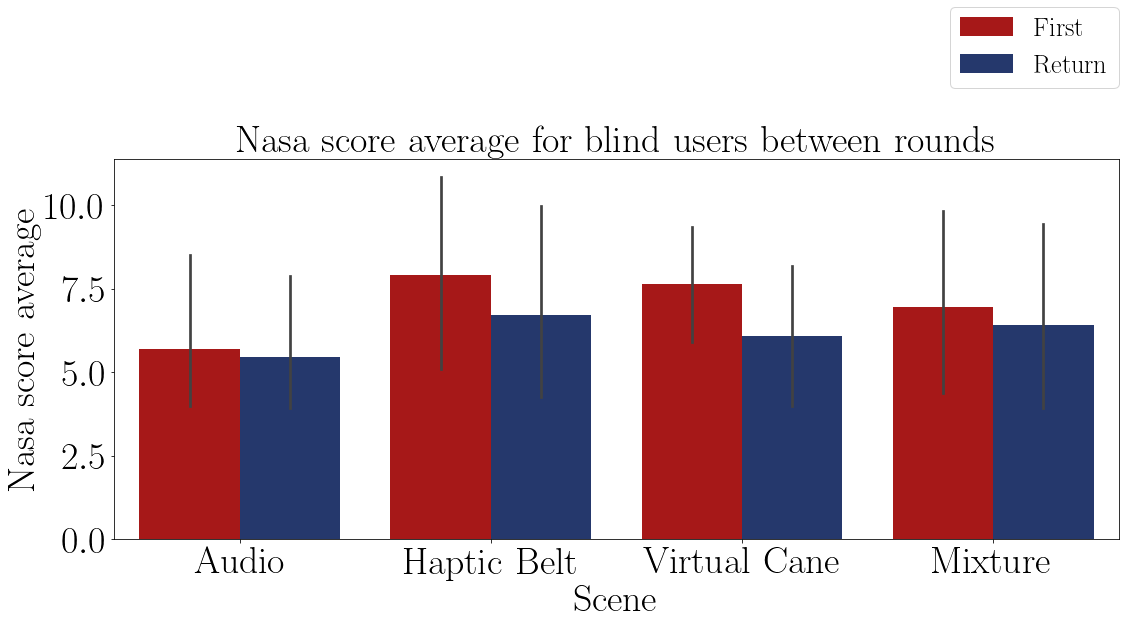
\includegraphics[width = 0.8\linewidth]{Resultados/Nasa/Figuras/png/barplot_nasa_avg_4_scene_blind.png}
        \subcaption{Blind participants.}
        \label{fig:barplot_nasa_avg_4_scene_blind}
    \end{minipage}
    \begin{minipage}{\textwidth}
        \centering
        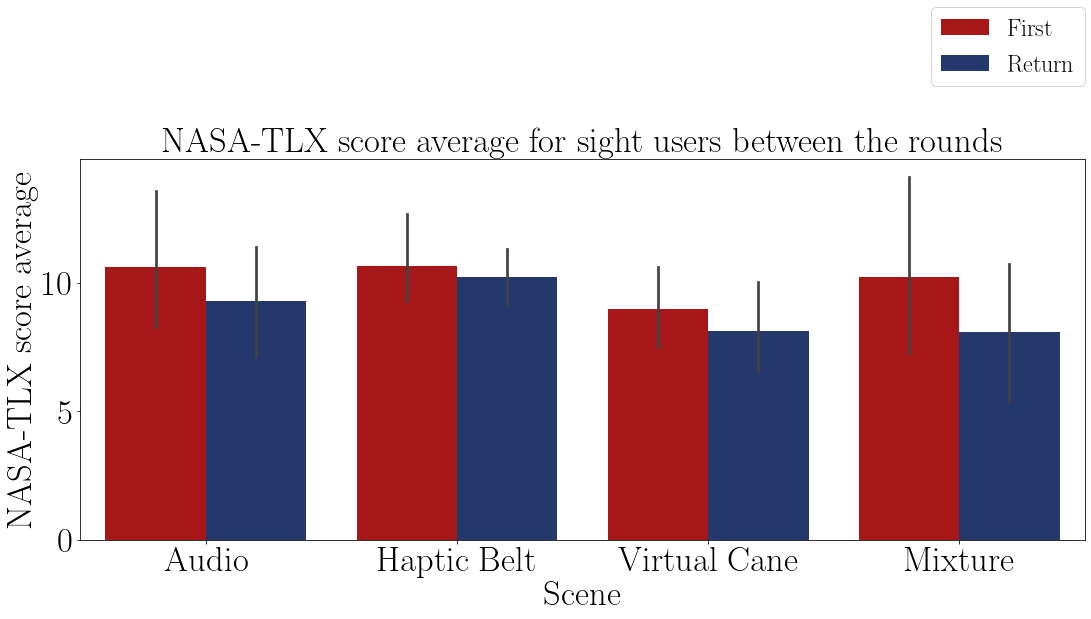
\includegraphics[width = 0.8\linewidth]{Resultados/Nasa/Figuras/png/barplot_nasa_avg_4_scene_sight.png}
        \subcaption{Sight participants.}
        \label{fig:barplot_nasa_avg_4_scene_sight}
    \end{minipage}
    \caption{Barplot of the NASA-TLX score on each method and round.}
    \label{fig:barplot_nasa_avg_4_scene}
\end{figure}
%\begin{figure}[!htb]
%    \centering
%    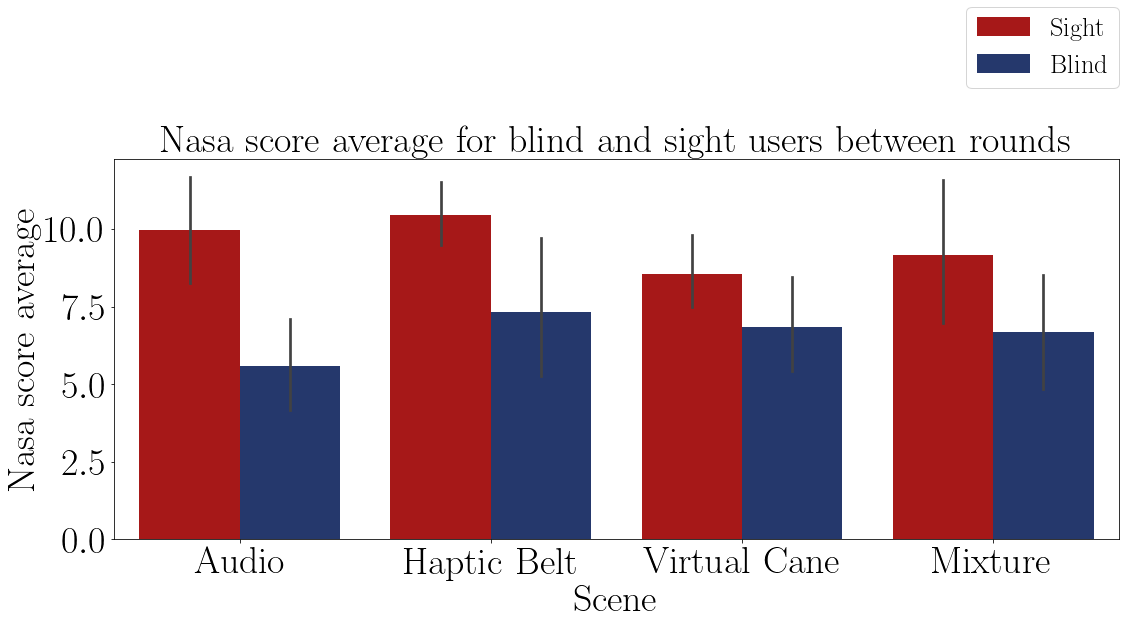
\includegraphics[width = 0.8\linewidth]{Resultados/Nasa/Figuras/png/barplot_nasa_avg_4_scene.png}
%    \caption{Barplot of the NASA-TLX score of both participants on each method.}
%    \label{fig:barplot_nasa_avg_4_scene}
%\end{figure}

Figures \ref{fig:boxplot_noBase_nasa_4_scene} and \ref{fig:boxplot_noBase_nasa_4_rounds} present the boxplots of NASA-TLX global score. Again, it is possible to see that sighted people usually give higher workload scores than blind ones. The influence of the round is approximately the same. But the order of preference of the methods are different.

\begin{figure}[!htb]
    \centering
    \begin{minipage}{0.45\textwidth}
        \centering
        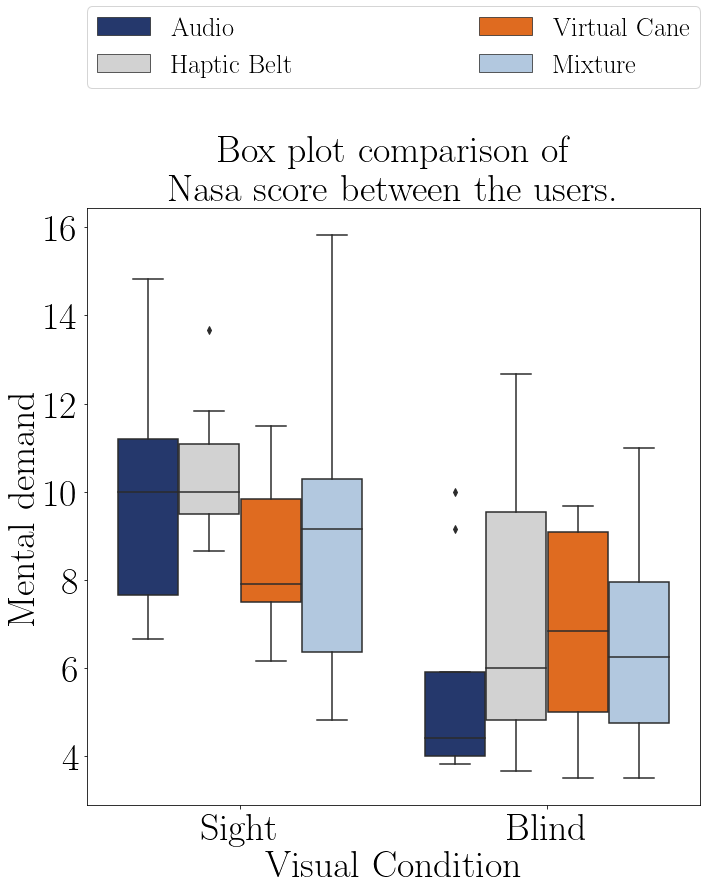
\includegraphics[width = 0.8\linewidth]{Resultados/Nasa/Figuras/png/boxplot_noBase_nasa_4_scene.png}
        \caption{Boxplot of the NASA-TLX score of the participants grouped by method.}
        \label{fig:boxplot_noBase_nasa_4_scene}
    \end{minipage}
    \begin{minipage}{0.45\textwidth}
        \centering
        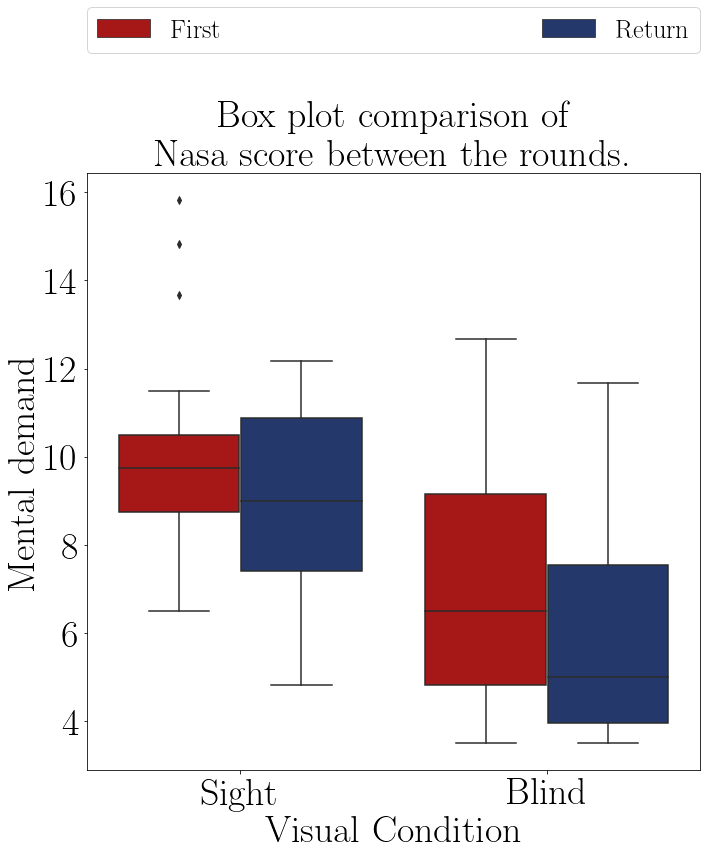
\includegraphics[width = 0.8\linewidth]{Resultados/Nasa/Figuras/png/boxplot_noBase_nasa_4_rounds.png}
        \caption{Boxplot of the NASA-TLX score of the participants grouped by round.}
        \label{fig:boxplot_noBase_nasa_4_rounds}
    \end{minipage}
\end{figure}

%The Table \ref{tab:nasa_average_group_noBase} shows the average NASA-TLX score of both samples and is possible to notice how the average perceived NASA-TXL average by the sight sample was also higher in every method.
%
%
\begin{table}[!htb]
\centering
\caption{Average NASA-TLX score grouped by participant and visual condition}
\label{tab:nasa_average_group_noBase}
\begin{tabular}{lrrrrrr}
\toprule
{} & Audio & \begin{tabular}[c]{@{}l@{}}Haptic\\ Belt\end{tabular} & \begin{tabular}[c]{@{}l@{}}Virtual\\ Cane\end{tabular} &  Mixture \\
Visual Condition &       &                                                       &                                                        &          \\
\midrule
Blind            &  5.58 &                                                  7.31 &                                                   6.85 &    6.688 \\
Sight            &  9.96 &                                                 10.46 &                                                   8.56 &    9.167 \\
\bottomrule
\end{tabular}
\end{table}


Figures \ref{fig:qqplot_nasa_avg_two_way_sight} and \ref{fig:residplot_nasa_avg_two_way_sight} bring the QQ plot and residual distribution of the data from sighted participants, showing that ANOVA can be used. The p-values for both groups are presented in Table \ref{tab:blocanova_nasa_avg_two_way_blind_sight}. It confirms the influence of the round for both sighted and blind people. In the case of the method, the p-value of ‘blind’ is lower than the threshold of 0.5, while that of ‘sighted’ is slightly higher.

\begin{table}
    \caption{Anova p-value for the mental demand average on each method'}
    \label{tab:blocanova_nasa_avg_two_way_blind_sight}
    \begin{minipage}{0.45\textwidth}
        \subcaption{Blind participants}
        
\centering
\begin{tabular}{ll}
\toprule
          Source & P-Value \\
\midrule
    \    Methods & 0.029** \\
     \    Rounds & 0.022** \\
\    Interaction &   0.814 \\
\bottomrule
\end{tabular}

    \end{minipage}
    \begin{minipage}{0.45\textwidth}
        \subcaption{Sight participants}
        
\centering
\begin{tabular}{ll}
\toprule
          Source & P-Value \\
\midrule
    \    Methods &   0.086 \\
     \    Rounds & 0.034** \\
\    Interaction &   0.688 \\
\bottomrule
\end{tabular}
    
    \end{minipage}
\end{table}


\begin{figure}[!htb]
    \centering
    \begin{minipage}{0.45\textwidth}
        \centering
        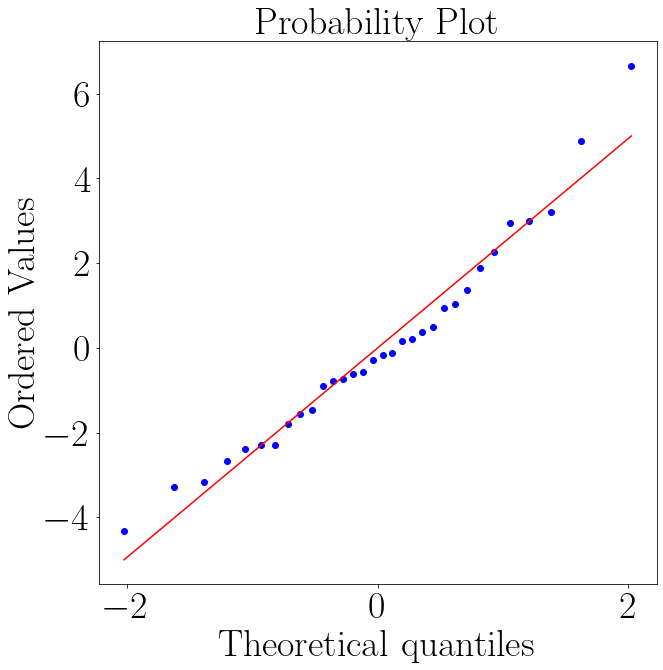
\includegraphics[width = 0.8\linewidth]{Resultados/Nasa/Figuras/png/qqplot_nasa_avg_two_way_sight.png}
        \caption{QQ plot of the NASA-TLX score of the sight participants on each method.}
        \label{fig:qqplot_nasa_avg_two_way_sight}
    \end{minipage}
    \begin{minipage}{0.45\textwidth}
        \centering
        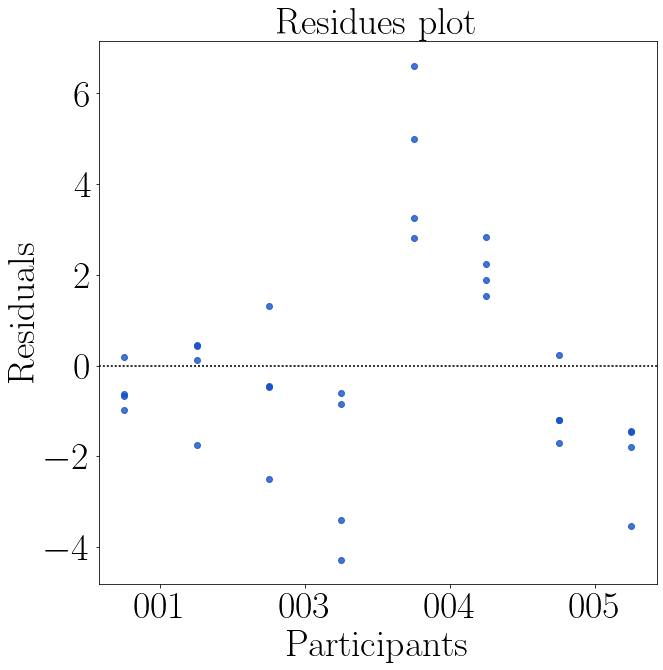
\includegraphics[width = 0.8\linewidth]{Resultados/Nasa/Figuras/png/residplot_nasa_avg_two_way_sight.png}
        \caption{Residual plot of the NASA-TLX score the sight participants on each method.}
        \label{fig:residplot_nasa_avg_two_way_sight}
    \end{minipage}
\end{figure}

%The Table \ref{tab:lsd_nasa_avg_two_way_sight} presents the conclusion of a pairwise Fisher LSD test of the previous ANOVA test and it shows that all the method had an effect in the NASA-TLX score.
%
%
\begin{table}[!htb]
\centering
\caption{Cross validation p-value for the NASA-TLX score average on each method for sighted users.}
\label{tab:lsd_nasa_avg_two_way_sight}
\begin{tabular}{rcllr}
\toprule
      \multicolumn{3}{c}{Method} &                          \multicolumn{2}{c}{Analysis} \\
\midrule
       Audio & $X$ & Haptic Belt &        $H_1 : \mu_{Audio} \ne \mu_{Haptic Belt}$ & ** \\
      Audio & $X$ & Virtual Cane &       $H_1 : \mu_{Audio} \ne \mu_{Virtual Cane}$ & ** \\
           Audio & $X$ & Mixture &            $H_1 : \mu_{Audio} \ne \mu_{Mixture}$ & ** \\
Haptic Belt & $X$ & Virtual Cane & $H_1 : \mu_{Haptic Belt} \ne \mu_{Virtual Cane}$ & ** \\
     Haptic Belt & $X$ & Mixture &      $H_1 : \mu_{Haptic Belt} \ne \mu_{Mixture}$ & ** \\
    Virtual Cane & $X$ & Mixture &     $H_1 : \mu_{Virtual Cane} \ne \mu_{Mixture}$ & ** \\
\bottomrule
\end{tabular}
\end{table}



%The Table \ref{tab:nasa_var_group} shows the average of the NASA-TLX score variation between the rounds. This table shows that the score variation from the “Audio” has the lower variation, and the rest are similar variations.

%
\begin{table}[!htb]
\centering
\caption{NASA-TLX score grouped by participant and visual Condition.}
\label{tab:nasa_var_group}
\begin{tabular}{lrrrrrr}
\toprule
{} &    Base &   Audio & \begin{tabular}[c]{@{}l@{}}Haptic\\ Belt\end{tabular} & \begin{tabular}[c]{@{}l@{}}Virtual\\ Cane\end{tabular} & Mixture \\
Visual Condition &         &         &                                                       &                                                        &         \\
\midrule
Blind            &  -0.9\% &  -0.3\% &                                                -1.2\% &                                                 -1.5\% &  -0.5\% \\
Sight            &  -0.0\% &  -1.3\% &                                                -0.4\% &                                                 -0.9\% &  -2.2\% \\
\bottomrule
\end{tabular}
\end{table}



%The Figures \ref{fig:qqplot_nasa_var_sight} and \ref{fig:residplot_nasa_var_sight} shows the distribution and variance of the NASA-TLX score variation of the Table \ref{tab:md_table_blind}. These Figures shows that the data are normally distributed and that the methods have a similar variance.

%The Table \ref{tab:blocanova_nasa_var_sight} shows the Anova test p-value of the NASA-TLX score of the "sight" sample between the guidance methods and it proves that there is no influence of the methods in the variation of score between the rounds. 

%
\begin{table}[!htb]
\centering
\caption{Anova p-value for the NASA score variation on each method for sighted users.}
\label{tab:blocanova_nasa_var_sight}
\begin{tabular}{lrrrrr}
\toprule
Source & P-Value \\
\midrule
Method &   0.274 \\
\bottomrule
\end{tabular}
\end{table}



%\begin{figure}[!htb]
%    \centering
%    \begin{minipage}{0.45\textwidth}
%        \centering
%        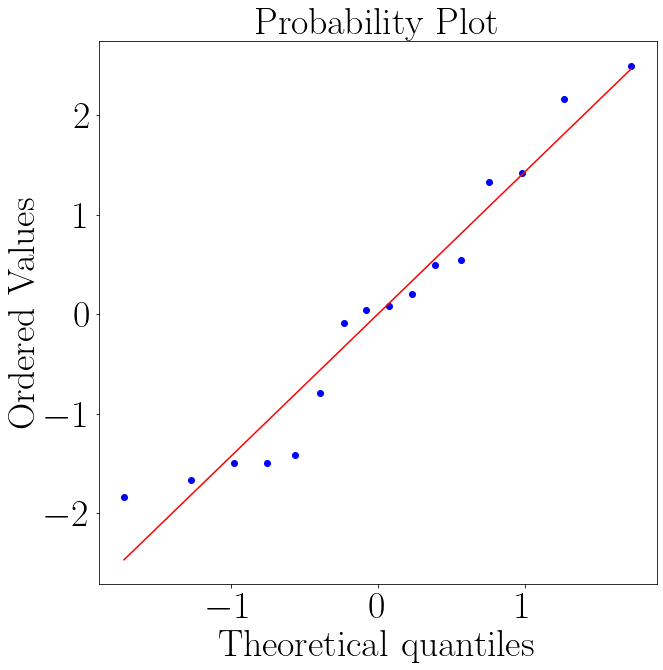
\includegraphics[width = 0.8\linewidth]{Resultados/Nasa/Figuras/png/qqplot_nasa_var_sight.png}
%        \caption{Residual plot of the variation NASA-TLX score of the blind participants on each method.}
%        \label{fig:qqplot_nasa_var_sight}
%    \end{minipage}
%    \begin{minipage}{0.45\textwidth}
%        \centering
%        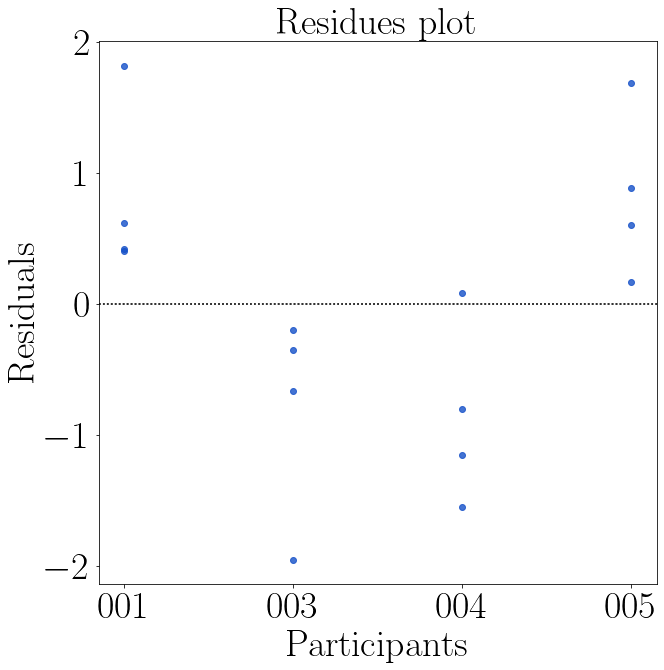
\includegraphics[width = 0.8\linewidth]{Resultados/Nasa/Figuras/png/residplot_nasa_var_sight.png}
%        \caption{Residual plot of the variation NASA-TLX score of the sighted participants on each method.}
%        \label{fig:residplot_nasa_var_sight}
%    \end{minipage}
%\end{figure}

%The Table \ref{tab:lsdbloc_mental_demand_var} presents the conclusion of a pairwise Fisher LSD test of the blind mental demand between all the guidance methods. The results show that all methods have similar variations.

%
\begin{table}[!htb]
\centering
\caption{Cross validation p-value for the mental demand variation on each method for blinded users.}
\label{tab:lsdbloc_mental_demand_var}
\begin{tabular}{rclr}
\toprule
      \multicolumn{3}{c}{Method} &                                       Analysis \\
\midrule
              Base & $X$ & Audio &           $H_1 : \mu_{Base} \ne \mu_{Audio}**$ \\
        Base & $X$ & Haptic Belt &         $H_0 : \mu_{Base} = \mu_{Haptic Belt}$ \\
       Base & $X$ & Virtual Cane &    $H_1 : \mu_{Base} \ne \mu_{Virtual Cane}**$ \\
            Base & $X$ & Mixture &         $H_1 : \mu_{Base} \ne \mu_{Mixture}**$ \\
       Audio & $X$ & Haptic Belt &    $H_1 : \mu_{Audio} \ne \mu_{Haptic Belt}**$ \\
      Audio & $X$ & Virtual Cane &       $H_0 : \mu_{Audio} = \mu_{Virtual Cane}$ \\
           Audio & $X$ & Mixture &            $H_0 : \mu_{Audio} = \mu_{Mixture}$ \\
Haptic Belt & $X$ & Virtual Cane & $H_0 : \mu_{Haptic Belt} = \mu_{Virtual Cane}$ \\
     Haptic Belt & $X$ & Mixture &  $H_1 : \mu_{Haptic Belt} \ne \mu_{Mixture}**$ \\
    Virtual Cane & $X$ & Mixture &     $H_0 : \mu_{Virtual Cane} = \mu_{Mixture}$ \\
\bottomrule
\end{tabular}
\end{table}



%To close up, according to the ANOVA test at Table \ref{tab:blocanova_nasa_avg_two_way_sight} the methods do not an effect on the score, but rounds do. The blind users felt an impact on both the method and the round.
%
%There is no influence in the tested methods in the participants NASA-TLX score variation, as shown in the Table \ref{tab:blocanova_nasa_var_sight}.

\FloatBarrier